\documentclass[12pt,a4paper,openright,twoside]{report}
\usepackage[italian,english]{babel}
\usepackage{fancyhdr}
\usepackage{indentfirst}
\usepackage{newlfont}
\usepackage{pdfpages}
\usepackage{abstract}
\usepackage{tabularx}
\usepackage{colortbl}
\usepackage{multirow}
\usepackage{graphicx}
\usepackage{listings}
\usepackage{subcaption}
\usepackage[hidelinks]{hyperref}
\definecolor{background}{HTML}{EEEEEE}
\lstdefinelanguage{json}{
    basicstyle=\footnotesize\ttfamily,
    numbers=left,
    numberstyle=\ttfamily,
    stepnumber=1,
    numbersep=8pt,
    showstringspaces=false,
    breaklines=true,
    backgroundcolor=\color{background}
}
\graphicspath{ {./images/} }
\oddsidemargin=30pt \evensidemargin=20pt
\pagestyle{fancy}\addtolength{\headwidth}{20pt}\setlength{\headheight}{15pt}
\renewcommand{\chaptermark}[1]{\markboth{\thechapter.\ #1}{}}
\renewcommand{\sectionmark}[1]{\markright{\thesection \ #1}{}}
\rhead[\fancyplain{}{\bfseries\leftmark}]{\fancyplain{}{\bfseries\thepage}}
\cfoot{}
\linespread{1.3}
\begin{document}
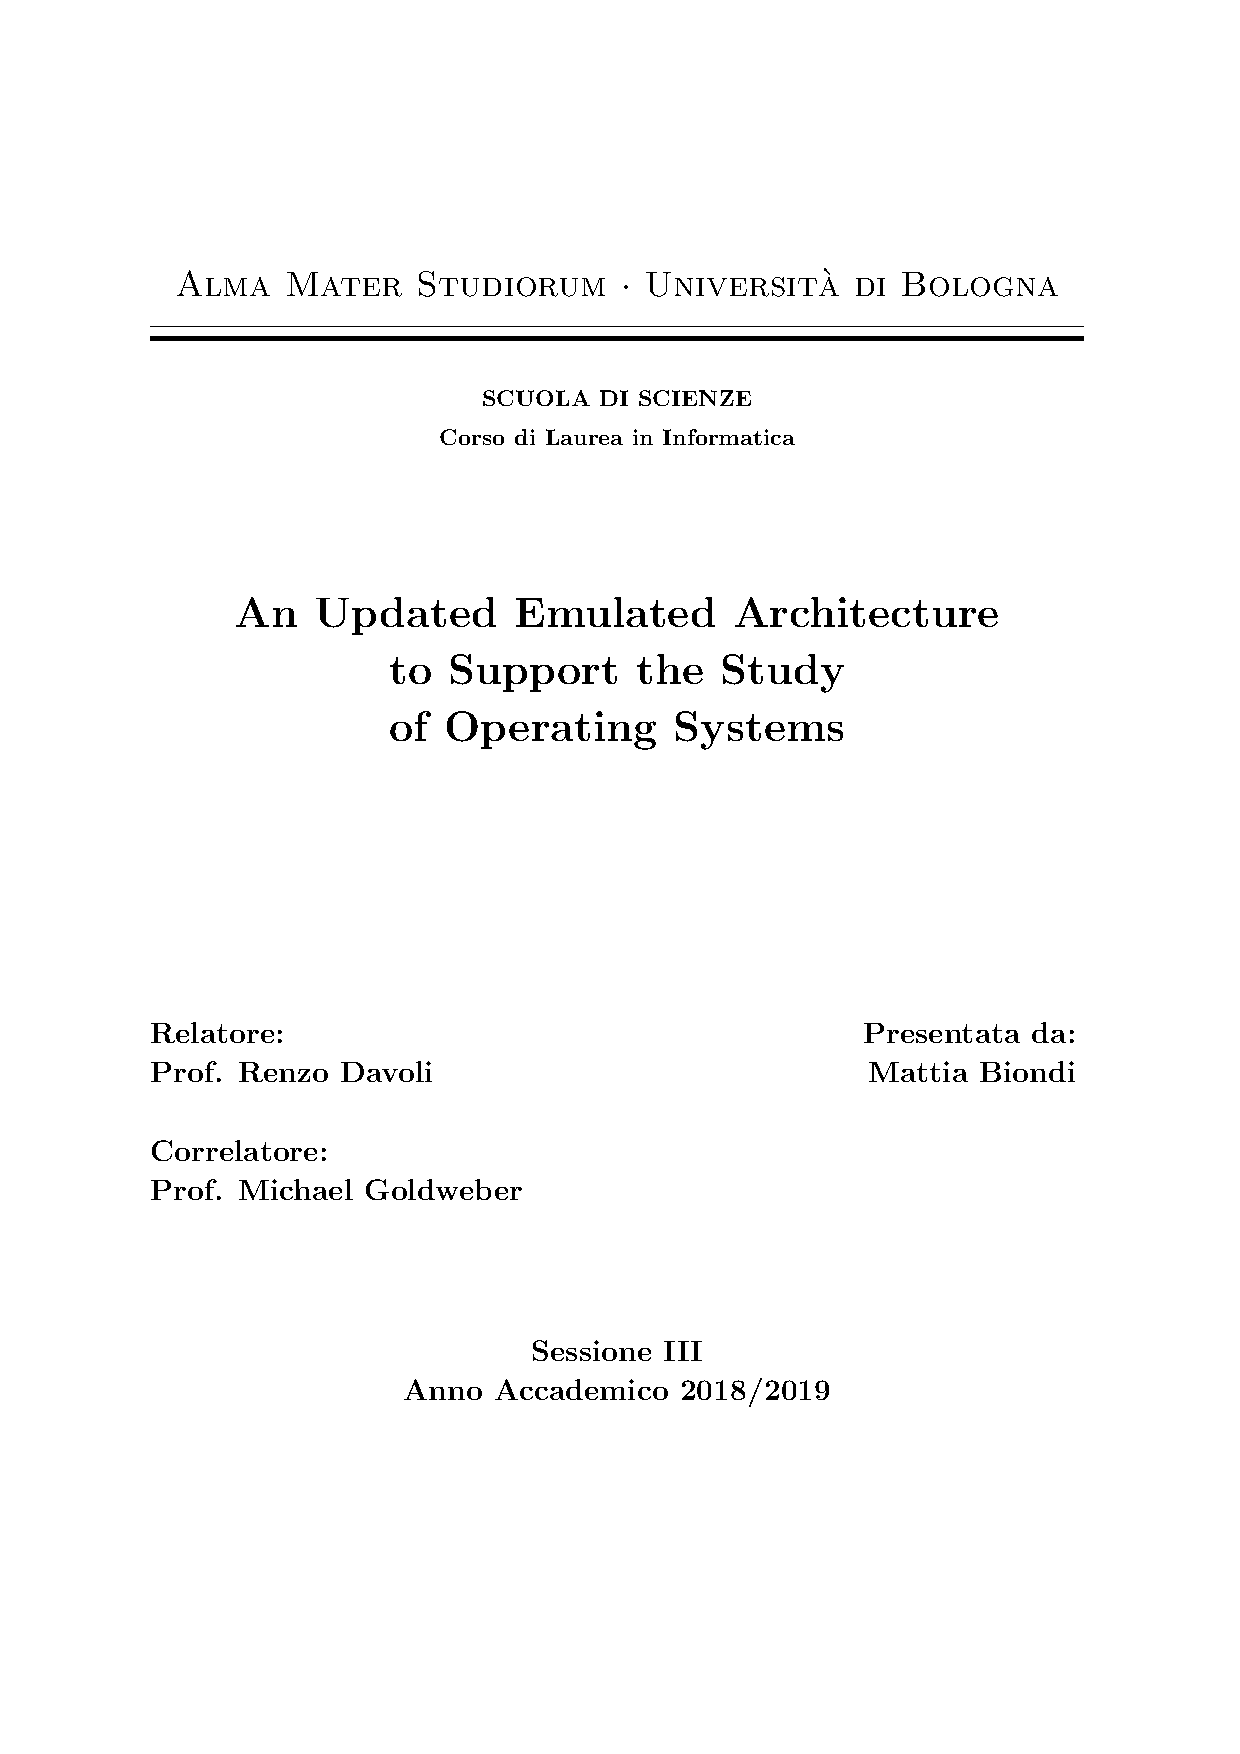
\includepdf[pages=-]{titlepage.pdf}
\clearpage{\pagestyle{empty}\cleardoublepage}
\begin{titlepage}
	\setcounter{page}{3}
	\thispagestyle{empty}
	\topmargin=6.5cm
	\raggedleft
	\large
	\em
	Agli amici di sempre,\linebreak
	alla mia famiglia,\linebreak
	che non mi ha mai impedito nulla,\linebreak
	e a Jas,\linebreak
	senza la quale non sarei qui oggi.
	\newpage
	\clearpage{\pagestyle{empty}\cleardoublepage}
\end{titlepage}
\begin{abstract}
	\pagenumbering{roman}
	One of the most effective ways to learn something new is by actively practising it, and there is---maybe---no better way to study an Operating Systems course than by building your own OS.

	However, it is important to emphasize how the realization of an operating system capable of running on a real hardware machine could be an overly complex and unsuitable task for an undergraduate student.
	Nonetheless, it is possible to use a simplified computer system simulator to achieve the goal of teaching Computer Science foundations in the University environment, thus allowing students to experience a quite realistic representation of an operating system.

	$\mu$MPS has been created for this purpose, a pedagogically appropriate machine emulator, based around the MIPS R2/3000 microprocessor, which features an accessible architecture that includes a rich set of easily programmable devices.
	$\mu$MPS has an almost two decades old historical development and the outcome of this following thesis is the third version of the software, dubbed $\mu$MPS3.
	This second major revision aims to simplify, even more, the complexity of the emulator in order to lighten the load of work required by the students during the OS design and implementation.
	Two of these simplifications are the removal of the virtual memory bit, which allowed address translation to be turned on and off, and the replacement of the tape device, used as storage devices, with a new flash drive device---certainly something more familiar to the new generation of students.

	Thanks to the employment of this software and the feedback received over the last decade, it has been possible to realize not just this following thesis, but also to develop some major improvements, which concern everything from the project building tools to the front-end, making $\mu$MPS a modern and reliable educational software.
\end{abstract}
\clearpage{\pagestyle{empty}\cleardoublepage}
\selectlanguage{italian}
\begin{abstract}
	\setcounter{page}{3}
	Uno dei metodi più efficaci per imparare qualcosa di nuovo è facendo pratica, e probabilmente, non esiste modo migliore di studiare un corso di Sistemi Operativi, se non scrivendo il proprio SO.
	È tuttavia necessario prendere atto di quanto la realizzazione di un sistema operativo, in grado di girare su una vera macchina hardware, sia un compito eccessivamente complesso e quasi inadeguato per uno studente universitario.
	Ciò non toglie che sia però possibile far uso di simulatori di sistemi semplificati rispetto alla realtà, al fine di riuscire nell'insegnamento dei fondamenti dell'Informatica in contesti universitari, permettendo così agli studenti di sperimentare con una rappresentazione di un sistema operativo abbastanza realistica.

	$\mu$MPS è stato sviluppato proprio a questo scopo, un emulatore di sistemi pedagogicamente appropriato, basato sul microprocessore MIPS R2/3000, e dotato di un'architettura accessibile e di una ricca lista di dispositivi facilmente programmabili.
	$\mu$MPS conta quasi vent'anni di sviluppo, ora aggiornato tramite la seguente tesi alla sua terza versione, chiamata $\mu$MPS3.
	Quest'ultimo aggiornamento mira a semplificare, ancor di più, la complessità dell'emulatore, al fine di alleggerire il carico di lavoro richiesto agli studenti durante lo sviluppo e l'implementazione del sistema operativo.
	Due di queste semplificazioni sono la rimozione del bit di memoria virtuale, che permetteva l'attivazione e la disattivazione della traduzione di indirizzi, e la sostituzione dei nastri, utilizzati come dispositivi di archiviazione, con delle nuove unità di memoria flash---certamente più familiari alla nuova generazione di studenti.

	Grazie all'utilizzo di questo software e dei feedback ricevuti, nel corso degli ultimi dieci anni, è stato possibile non solo realizzare la seguente tesi, ma anche apportare alcune importanti migliorie che riguardano tutti i campi, dagli strumenti di compilazione del progetto alla parte front-end, rendendo così $\mu$MPS un software pedagogico moderno e affidabile.
\end{abstract}
\clearpage{\pagestyle{empty}\cleardoublepage}
\selectlanguage{english}
\tableofcontents
\addtocontents{toc}{\protect\thispagestyle{empty}}
\listoffigures
\clearpage{\pagestyle{empty}\cleardoublepage}
\listoftables
\clearpage{\pagestyle{empty}\cleardoublepage}
\lstlistoflistings
\clearpage{\pagestyle{empty}\cleardoublepage}

\chapter*{Notational Conventions}
\begin{itemize}
	\item Words being defined are \textit{italicized};
	\item A \texttt{typewriter-like typeface} is used for memory addresses, machine registers, instructions, file names, identifiers, and code fragments;
	\item Memory addresses and operation codes are given in hexadecimal and displayed in big-endian format;
	\item Bits of storage are numbered right-to-left, starting with 0;
	\item All diagrams illustrating memory are going from low addresses to high addresses, using a left to right, bottom to top orientation.
\end{itemize}

\clearpage{\pagestyle{empty}\cleardoublepage}
\pagenumbering{arabic}
\chapter{Introduction}
\lhead[\fancyplain{}{\bfseries\thepage}]{\fancyplain{}{\bfseries\rightmark}}

\section{Background}
The study and the consequent implementation of how an operating system works is, by now, a long-established and consolidated practice in many Computer Science curriculum.
It is, actually, one of the crucial components of a computer and it is responsible for ensuring its basic operations, by coordinating and managing the system resources like processor, memory, devices and processes, thus allowing hardware and software to interface each other.

This is probably the first real example of ``big project'' which students should experience, thanks to the complex intercommunication system that has to exist between the different components of the machine, and the study of it allows to comprehend the most common software engineering practices.

The approach on practical contexts is essential to fully understand how a machine works behind the theoretical notions studied in the early stages of the course of study, and it is usually followed by the debate of which is the best teaching choice concerning processor architectures.

Obviously, there is not only one way of how a central processor unit can be implemented, and while older realizations---although applicable for educational purposes---are now obsolete and incompatible with current platforms, modern ones are designed to achieve high speed and quality, which makes them overly complex and unsuitable for the pedagogic experience.

Over the years, the MIPS architecture has become one of the landmarks in this teaching choice due to its clean and elegant instruction set, despite being excessively convoluted to student's perception, because of the high level of details obscuring the basic underlying features of it.
A potential solution to this problem is the adoption of a simplified computer system simulator, like $\mu$MPS, to bring together an adequate level of understanding and a realistic representation of a real operating system.

\section{History of $\mu$MPS}
$\mu$MPS is based on the machine emulator \textit{MPS} \cite{mps}, designed and realized by Professor Renzo Davoli and one of his graduate students Mauro Morsiani, in the late 1990s at the University of Bologna.

MPS, in turn, was created with the intention of recreating the same asset that a previous, fell out of use, machine emulator provided.
\textit{CHIP} \cite{chip_1, chip_2} (Cornell Hypothetical Instruction Processor) was its name, developed at the Cornell University and based on a made-up architecture that was a cross between a \textit{PDP-11} and an \textit{IBM S/370}.
The operating system designated to run on it was named \textit{HOCA} \cite{hoca}, a three phase/layer project, named after the Turkish word \textit{hoca} (``schoolmaster'' or ``giver of good advice'') which was proposed by one of its author, Özalp Babaoğlu, who is currently teaching at the University of Bologna.

The initial purpose of MPS was to bring back to life the layout and implementation experience of an operating system through an educational emulator, which could be run on real hardware.
This practice was already possible in the past years when the architecture of the processor studied was the same available on real machines, but it has gone lost through the years because of the high-speed development of new and more complex technologies used on physical implementations.

MPS was able to emulate the MIPS R3000 processor along with five other different device categories: disks, tapes, network adapters, printers and terminals.
In addition, the Hoca project was updated and adapted to the new MPS architecture.

The concerned CPU was genuinely emulated together with its complex virtual memory management system, which was the main subject of the feedback received during class testing of MPS as a pedagogical tool at the University of Bologna and Xavier University, in an undergraduate operating systems courses, taught respectively by Renzo Davoli and Michael Goldweber.

It was tested through the implementation of a direct descendant of HOCA, \textit{Kaya} \cite{kaya}, one of the variety of graduate-level projects that the emulator can support.

The urge of simplification led to the creation of $\mu$MPS, virtually identical to MPS but with the addition of a virtual memory management subsystem which had to resemble as much as possible to the conceptual one found in popular introductory OS texts.
The only other difference was the new novice-friendly graphical user interface, significantly improved again in 2011 by Tomislav Jonjic during the development of the first major revision of the emulator, $\mu$MPS2 \cite{umps2}, which also implemented the support to up to sixteen MIPS R3000-style processors.

\section{$\mu$MPS3}
More than ten years have passed since the first release of $\mu$MPS and as many have passed from the moment it has been developed into a consolidated educational tool.
At its peak, it was adopted by more than 50 institutions, proving that its initial purpose had been achieved.

Over time, this number has decreased, showing that a refresh of the tool was needed to regain the attention of new generations of OS instructors.
The students' observations during this period of use were essential to understand which of these further changes were required to give $\mu$MPS a new life as an useful pedagogical tool.

Some examples of these modifications would be the structure and management system of both physical and virtual memory, a nuance probably still too complex and confusing, which could feel like a regression, since the attempt to simplify it has led to the removal of the VM bit.
This was originally introduced in the first version of $\mu$MPS, as a distinctive feature from its predecessor MPS.
Virtual memory segmentation has been eliminated too, since it is considered as legacy in current architectures, making its implementation an unnecessary complication for the students.

There are also other changes related to the passage of the years, such as the replacement of memory tapes with flash drive devices, also known as ``USB sticks'', ``SD Cards'' or even ``SSDs''.
Tapes are probably still studied in their operation nowadays, but they cannot be found in today's practical contexts, and therefore it could be difficult to understand for the new generation of students, who cannot find a match in current technological implementations.

Another consequence of the update of $\mu$MPS has been the shift from the historical and well established Autotools to a more current building tool, CMake, that speeds up the compilation process in addition to simplifying the structure of the project.
It also fits best with the current graphical user interface of the emulator, originally built upon Qt4, which also undergoes to the migration to the new version, Qt5.

These and more changes are collected together in a major release of the project, $\mu$MPS3, consequently bringing even more reliability in terms of pedagogical tool.

Due to implementation aspects---unlike its predecessor $\mu$MPS2---this new version is not backward compatible with older versions.

\section{Structure of the Document}
This thesis will primarily focus on the modifications made on the previous version of the emulator, their implementation and the reasons to do it.
This document is not intended to be used as a substitute of the manual \textit{$\mu$MPS3 Principles of Operation} \cite{pops}, but only as an accompanying guide to understand how the two versions differ from each other.

This first chapter aims to give a brief overview of why tools like $\mu$MPS are needed, its history to date and the considerations on why an update was necessary.

Chapter 2 and 3 will respectively describe the new memory management, as both physical and virtual ones have been updated, and the new exception handling mechanism.
Both current and previous implementations will be compared in every aspect.

Chapter 4 will explain the advanced feature of the multiprocessor support.
The CPUs initialization has been updated to comply with the new exception handling.

Chapter 5 is an introduction of the new flash device, which takes over tapes.
The reasons why this replacement was necessary are described in the first part of the chapter, while the rest of the chapter illustrates its creation and its usage.

Chapter 6 is the less technical one, since it describes the migration from the old project building tool to the new one, and the renewal of the graphical user interface.

Finally, chapter 7 will provide a brief summary of the topics covered by this thesis and the reasons for the changes made.
A shortlist of possible future implementation is also given.

\chapter{Memory Management}
\lhead[\fancyplain{}{\bfseries\thepage}]{\fancyplain{}{\bfseries\rightmark}}
Like for the two prior versions, the memory subsystem of $\mu$MPS3 is divided into two views: physical and virtual.
Both parts have undergone significant modifications in this major revision, and they will be described in detail in this chapter, alongside their old versions and respective changes.

The main reasons for the modifications made are the further simplification of the work required by the user for the kernel implementation and the better clarification of the internal view of the emulator memory, which, in the past, have caused some difficulties to the students.

\section{Physical Memory}
\label{chap:physical_memory}
The physical address space is divided into two big areas [\autoref{fig:physical_memory}]: a \textit{BIOS reserved space}, from address \texttt{0x0000.0000} to \texttt{0x2000.0000}, and the \textit{installed RAM}, from address \texttt{0x2000.0000} (\texttt{RAMBASE}) to \texttt{RAMTOP}.

This last value is calculated upon the one retrieved from the configuration file, settable from the configuration dialog of the machine in the front-end emulator, which goes from a minimum of 8 to a maximum of 512 memory frames.
Being the size of each frame 4 kilobyte, $\mu$MPS3 can have from 32KB up to 2MB of installed RAM.
Hence, the value of \texttt{RAMTOP} range from \texttt{0x2000.8000} to \texttt{0x2020.0000}.

\begin{figure}[ht]
	\centering
	\renewcommand{\arraystretch}{0.755}
	\begin{tabular}{cl}
		                                                           & \multirow{2}{*}{\texttt{0xFFFF.FFFF}} \\ \cline{1-1}
		\multicolumn{1}{|c|}{\multirow{2}{*}{\cellcolor{gray}}}    &                                       \\ [-1ex]
		\multicolumn{1}{|c|}{\cellcolor{gray}}                     & \multirow{2}{*}{\texttt{RAMTOP}}      \\ \cline{1-1}
		\multicolumn{1}{|c|}{\multirow{4}{*}{installed RAM}}       &                                       \\
		\multicolumn{1}{|c|}{}                                     &                                       \\
		\multicolumn{1}{|c|}{}                                     &                                       \\
		\multicolumn{1}{|c|}{}                                     & \multirow{2}{*}{\texttt{0x2000.0000}} \\ \cline{1-1}
		\multicolumn{1}{|c|}{\multirow{2}{*}{BIOS reserved space}} &                                       \\
		\multicolumn{1}{|c|}{}                                     & \multirow{2}{*}{\texttt{0x0000.0000}} \\ \cline{1-1}
		\multicolumn{1}{l}{}                                       &
	\end{tabular}
	\caption{Physical Memory}
	\label{fig:physical_memory}
\end{figure}

\subsection{BIOS Reserved Space}
\label{chap:bios_reserved_space}
The first big area of the memory [\autoref{fig:kernel_reserved_space}] is reserved for:
\begin{itemize}
	\item the \textit{Execution BIOS Services} \cite{pops}, which lay in a read-only segment from address \texttt{0x0000.0000} to \texttt{EXECTOP}.
	      This latter value is calculated upon the size of the Execution BIOS Services code;
	\item the \textit{BIOS Data Page}, from address \texttt{0x0FFF.F000} (\texttt{BIOSDATABASE}) to \texttt{0x1000.0000}.
	      This is the same 4KB area that was used to be called ``ROM Reserved Frame'' [\autoref{chap:rom_reserved_frame}] in $\mu$MPS2, which has been renamed and moved.
	      However, it still serves as an interface between the BIOS handlers [\autoref{chap:bios_exception_handlers}] and the user-implemented kernel.
	      See \autoref{chap:bios_data_page} for more information regarding how this read/writable area segment has been updated;
	\item the \textit{Bus Register Area}, from address \texttt{0x1000.0000} to \texttt{0x1000.002C}: a 11 word area containing various fields used in the lifetime cycle of $\mu$MPS3 to properly work.
	      Some of them are read-only and calculated at boot/reset time, while others are read/writable.
	      See \cite{pops} for more information regarding this area;
	\item the \textit{Installed Devices Bit Map}, from address \texttt{0x1000.002C} to \\ \texttt{0x1000.0040}: a read-only five word area indicating which devices are actually installed and where \cite{pops};
	\item the \textit{Interrupting Devices Bit Map}, from address \texttt{0x1000.0040} to \\ \texttt{0x1000.0054}: a read-only five word area indicating which devices have an interrupt pending \cite{pops};
	\item the \textit{Devices Registers Area}, from address \texttt{0x1000.0054} to \texttt{0x1000.02D4} (\texttt{DEVTOP}): a 160 word area (number of interrupt lines (8) $\times$ devices per interrupt line (5) $\times$  words per register (4)).
	      See \cite{pops} for more information, or \autoref{tab:device_register_layout} for an example of one device register;
	\item the \textit{Bootstrap BIOS Services} \cite{pops}, which lay in a read-only segment from address \texttt{0x1FC0.0000} to \texttt{BOOTTOP}.
	      This latter value is calculated upon the size of the Bootstrap BIOS Services code.
\end{itemize}
\begin{figure}[ht]
	\centering
	\begin{tabular}{cl}
		\multicolumn{1}{l}{}                                                & \multirow{2}{*}{\texttt{0x2000.0000}} \\ \cline{1-1}
		\multicolumn{1}{|l|}{\cellcolor{gray}}                              &                                       \\ [-3ex]
		\multicolumn{1}{|l|}{\cellcolor{gray}}                              & \multirow{2}{*}{\texttt{BOOTTOP}}     \\ \cline{1-1}
		\multicolumn{1}{|c|}{\multirow{2}{*}{Bootstrap BIOS Services}}      &                                       \\ [-1ex]
		\multicolumn{1}{|c|}{}                                              & \multirow{2}{*}{\texttt{0x1FC0.0000}} \\ \cline{1-1}
		\multicolumn{1}{|l|}{\multirow{2}{*}{\cellcolor{gray}}}             &                                       \\ [-3ex]
		\multicolumn{1}{|l|}{\cellcolor{gray}}                              & \multirow{2}{*}{\texttt{DEVTOP}}      \\ \cline{1-1}
		\multicolumn{1}{|c|}{\multirow{2}{*}{Devices Registers Area}}       &                                       \\ [-1ex]
		\multicolumn{1}{|c|}{}                                              & \multirow{2}{*}{\texttt{0x1000.0054}} \\ \cline{1-1}
		\multicolumn{1}{|c|}{\multirow{2}{*}{Interrupting Devices Bit Map}} &                                       \\ [-1ex]
		\multicolumn{1}{|c|}{}                                              & \multirow{2}{*}{\texttt{0x1000.0040}} \\ \cline{1-1}
		\multicolumn{1}{|c|}{\multirow{2}{*}{Installed Devices Bit Map}}    &                                       \\ [-1ex]
		\multicolumn{1}{|c|}{}                                              & \multirow{2}{*}{\texttt{0x1000.002C}} \\ \cline{1-1}
		\multicolumn{1}{|c|}{\multirow{2}{*}{Bus Register Area}}            &                                       \\ [-1ex]
		\multicolumn{1}{|c|}{}                                              & \multirow{2}{*}{\texttt{0x1000.0000}} \\ \cline{1-1}
		\multicolumn{1}{|c|}{\multirow{2}{*}{BIOS Data Page}}               &                                       \\ [-1ex]
		\multicolumn{1}{|c|}{}                                              & \multirow{2}{*}{\texttt{0x0FFF.F000}} \\ \cline{1-1}
		\multicolumn{1}{|l|}{\multirow{2}{*}{\cellcolor{gray}}}             &                                       \\ [-3ex]
		\multicolumn{1}{|l|}{\cellcolor{gray}}                              & \multirow{2}{*}{\texttt{EXECTOP}}     \\ \cline{1-1}
		\multicolumn{1}{|c|}{\multirow{2}{*}{Execution BIOS Services}}      &                                       \\ [-1ex]
		\multicolumn{1}{|c|}{}                                              & \multirow{2}{*}{\texttt{0x0000.0000}} \\ \cline{1-1}
		\multicolumn{1}{l}{}                                                &
	\end{tabular}
	\caption{Structure of the BIOS Reserved Space}
	\label{fig:kernel_reserved_space}
\end{figure}
Any attempt to access an undefined memory area (\texttt{EXECTOP...0x0FFF.F000}, \texttt{DEVTOP...0x1FC0.0000}, \texttt{BOOTTOP...0x2000.0000}) will generate a \textit{Bus Error exception} [\autoref{chap:exception_handling}].

Note: the memory area between address \texttt{0x1000.02D4} (\texttt{DEVTOP}) and \texttt{0x1FC0.0000} is not completely undefined [section 7.3 of the old manual \cite{old_pops}].

\subsection{RAM Space}
The maximum \texttt{RAMTOP} value actually settable is \texttt{0x2020.0000}.
However, since $\mu$MPS3 uses 32-bit addresses, it could support up to [$2^{32}$ - \texttt{RAMBASE}] $\simeq$ 3.5GB of RAM.
The 2MB graphical user interface limitation is imposed because, while it seems a ridiculously small amount of memory in today's ordinary systems, it is, actually, a lot more than has ever been required in all these years of $\mu$MPS use.

This area will hold:
\begin{itemize}
	\item the code (\textit{text}), global variables/structures (\textit{data}), and stack(s) of the operating system;
	\item enough space for the ``frame pool'' to be used for the text, data and stacks of the user processes during virtual memory management.
\end{itemize}
As for the previous big area, any attempt to access the undefined memory area laying from \texttt{RAMTOP} up to \texttt{0xFFFF.FFFF} will generate a Bus Error exception.

\section{Virtual Memory}
While the physical one is divided into two big areas, the virtual memory subsystem is logically split into four units [\autoref{fig:virtual_memory}]:
\begin{itemize}
	\item \textit{kseg0}, from address \texttt{0x0000.0000} to \texttt{0x2000.0000}: a 0.5GB address space dedicated to the BIOS Reserved Space [\autoref{chap:bios_reserved_space}];
	\item \textit{kseg1}, from address \texttt{0x2000.0000} to \texttt{0x4000.0000}: a 0.5GB address space dedicated to the text, data and stacks of the OS;
	\item \textit{kseg2}, from address \texttt{0x4000.0000} to \texttt{0x8000.0000}: a 1GB address space dedicated to the text, data and stacks of the OS;
	\item \textit{kuseg}, from address \texttt{0x8000.0000} to \texttt{0xFFFF.FFFF}: a 2GB address space dedicated to the text, data and stacks of the user processes;
\end{itemize}

Since the \textit{TLB Floor Address} [\autoref{chap:tlb_floor_address}] minimum value is \texttt{0x4000.0000}, kseg0 and kseg1 are always referring to physical memory space.

\begin{figure}[h]
	\centering
	\renewcommand{\arraystretch}{0.57}
	\begin{tabular}{cl}
		\multicolumn{1}{m{3cm}}{}                    & \multirow{2}{*}{\texttt{0xFFFF.FFFF}} \\ \cline{1-1}
		\multicolumn{1}{|c|}{\multirow{4}{*}{kuseg}} &                                       \\
		\multicolumn{1}{|c|}{}                       & \multirow{2}{*}{}                     \\
		\multicolumn{1}{|c|}{}                       &                                       \\
		\multicolumn{1}{|c|}{}                       & \multirow{2}{*}{\texttt{0x8000.0000}} \\ \cline{1-1}
		\multicolumn{1}{|c|}{\multirow{4}{*}{kseg2}} &                                       \\
		\multicolumn{1}{|c|}{}                       & \multirow{2}{*}{}                     \\
		\multicolumn{1}{|c|}{}                       &                                       \\
		\multicolumn{1}{|c|}{}                       & \multirow{2}{*}{\texttt{0x4000.0000}} \\ \cline{1-1}
		\multicolumn{1}{|c|}{\multirow{2}{*}{kseg1}} &                                       \\
		\multicolumn{1}{|c|}{}                       & \multirow{2}{*}{\texttt{0x2000.0000}} \\ \cline{1-1}
		\multicolumn{1}{|c|}{\multirow{2}{*}{kseg0}} &                                       \\
		\multicolumn{1}{|c|}{}                       & \multirow{2}{*}{\texttt{0x0000.0000}} \\ \cline{1-1}
		\multicolumn{1}{l}{}                         &
	\end{tabular}
	\caption{Virtual Memory Structure}
	\label{fig:virtual_memory}
\end{figure}
Despite their name, these four sections are not real segments, since virtual memory segmentation has been removed in $\mu$MPS3.
However, they are called like this for traditional reasons, as their size and their label are the same as the areas from the original MIPS address space.

The first 2GB of the address space, corresponding to all the addresses below \texttt{0x8000.0000}, are reserved only to kernel-mode access, therefore, any attempt to access them while the processor is in user-mode will cause the raising of an \textit{Address Error} [\autoref{chap:exception_handling}].

The other half of the address space is dedicated to user processes, and each one ``sees'' its own logical version.
The kuseg of one process is separated from the one of another process by a unique number called \textit{ASID} (Address Space Identifier) \cite{pops}.

\subsection{TLB Floor Address}
\label{chap:tlb_floor_address}
The TLB Floor Address is a new parameter implemented in $\mu$MPS3, responsible for indicating which addresses from a certain value on are considered logical, and therefore subject to \textit{address translation}---the process of mapping logical addresses to physical ones.
By doing this, the processes perceive more physical memory than the one actually available, recreating an abstract view of the address space.

This parameter can be chosen directly from the configuration dialog in the emulator front-end, as Figure \ref{fig:tlb_floor_address} shows:
\begin{figure}[h]
	\centering
	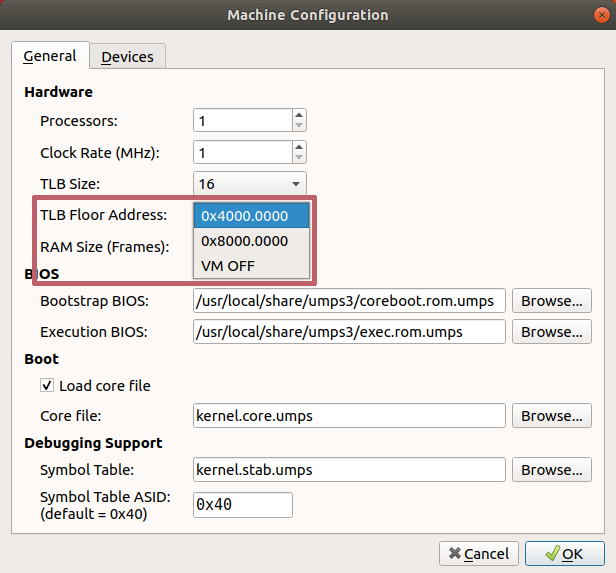
\includegraphics[scale=0.68]{tlb_floor_address}
	\caption{TLB Floor Address}
	\label{fig:tlb_floor_address}
\end{figure}

The last option, \texttt{VM OFF}, is internally declared as \texttt{0xFFFF.FFFF}: since it is not possible to access to an address above this value, the entire physical memory is necessarily below it, and therefore, an address translation could never happen.

\section{Previous Implementation}
The physical address space was substantially equal to the new one, except for the moving and renaming of the new ``BIOS Data Page''.

On the other hand, the virtual memory was implemented through a segmented-paged scheme.
Hence, a new abstraction layer was laid on the whole physical memory structure, subdividing it into three big segments [\autoref{fig:old_virtual_memory}]:
\begin{itemize}
	\item \textit{ksegOS}, from address \texttt{0x0000.0000} to \texttt{0x8000.0000}: a 2GB segment reserved for the text, data and stacks of the OS, along with all the structures sitting in the BIOS reserved space up to address \texttt{0x2000.0000};
	\item \textit{kUseg2}, from address \texttt{0x8000.0000} to \texttt{0xC000.0000}: a 1GB logical address space reserved for the text, data and stacks of the user processes;
	\item \textit{kUseg3}, from address \texttt{0xC000.0000} to \texttt{0xFFFF.FFFF}: another 1GB logical address space reserved for the use of user-mode processes.
\end{itemize}

\begin{figure}[h]
	\centering
	\begin{tabular}{cl}
		\multicolumn{1}{m{3cm}}{}                     & \multirow{2}{*}{\texttt{0xFFFF.FFFF}} \\ \cline{1-1}
		\multicolumn{1}{|c|}{\multirow{2}{*}{kUseg3}} &                                       \\
		\multicolumn{1}{|c|}{}                        & \multirow{2}{*}{\texttt{0xC000.0000}} \\ \cline{1-1}
		\multicolumn{1}{|c|}{\multirow{2}{*}{kUseg2}} &                                       \\
		\multicolumn{1}{|c|}{}                        & \multirow{2}{*}{\texttt{0x8000.0000}} \\ \cline{1-1}
		\multicolumn{1}{|c|}{\multirow{4}{*}{ksegOS}} &                                       \\
		\multicolumn{1}{|c|}{}                        & \multirow{4}{*}{}                     \\
		\multicolumn{1}{|c|}{}                        &                                       \\
		\multicolumn{1}{|c|}{}                        & \multirow{2}{*}{\texttt{0x0000.0000}} \\ \cline{1-1}
		\multicolumn{1}{l}{}                          &
	\end{tabular}
	\caption{Old Virtual Memory Structure}
	\label{fig:old_virtual_memory}
\end{figure}

As for the new version, all the addresses below \texttt{0x8000.0000} were reserved to kernel-mode access only.

Whether this subdivision was active or not was controlled by the \textit{VM bit}.
With the VM bit off, no particular actions were required when accessing the memory space.
Instead, when the VM bit was on, all the address above \texttt{0x2000.0000} were considered logical and sent to the \textit{MMU} for address translation.

The VM bit was originally introduced in the first version of $\mu$MPS, with the intent of simplifying the complex virtual memory management system of the MIPS R3000 microprocessor.
The activation and deactivation of it was accomplished through the system control coprocessor \textit{CP0}.

It provides a 32-bit \textit{Status} register that controls various aspects of the emulator, described in details in \cite{pops}.
Along with the current options set of the register, it also provided the possibility, by using bitwise operations, to control the status of the VM bit: it was implemented as a 3-slot deep bit stack (current, previous, previous of previous) which was pushed or popped depending on whether an exception was raised or an interrupted execution stream was restarted [section 3.2 and subsection 6.2.1 of \cite{old_pops}].

The virtual address translation process went through a significant change in this major revision: the formal segment table [subsections 4.3.1 of \cite{old_pops}], introduced in the first implementation of $\mu$MPS, have been removed.
Consequently, only TLB table formats remain implemented, resulting in a simpler procedure for the users \cite{pops}.

During the implementation of a new feature of the emulator, the VM bit has been completely removed too.

\section{VM Bit Removal}
\label{chap:vm_bit_removal}
The VM bit removal is one of the main features of $\mu$MPS3: the push/pop system has been removed, and the three bits previously reserved for it are now completely ignored.
Hence, from now on, the virtual memory is conceptually always on.
This means that all the addresses above a certain value are considered logical and therefore, subject to address translation.
This specific value, while in previous version was fixed at \texttt{0x2000.0000}, is now contained in a variable called TLB Floor Address [\autoref{chap:tlb_floor_address}].

The TLB Floor Address value is stored in the Bus Register Area, thereby adding one word to the ten word area of the previous version [\autoref{tab:bus_register_area}]:
\begin{table}[h]
	\centering
	\begin{tabular}{|c|c|}
		\hline
		Physical Address     & Field Name                                    \\ \hline\hline
		\texttt{0x1000.0028} & TLB Floor Address                             \\ \hline
		\texttt{0x1000.0024} & Time Scale                                    \\ \hline
		\texttt{0x1000.0020} & Interval Timer                                \\ \hline
		\texttt{0x1000.001C} & Time of Day Clock - Low                       \\ \hline
		\texttt{0x1000.0018} & Time of Day Clock - High                      \\ \hline
		\texttt{0x1000.0014} & Installed Bootstrap BIOS Services Size        \\ \hline
		\texttt{0x1000.0010} & Bootstrap BIOS Services Base Physical Address \\ \hline
		\texttt{0x1000.000C} & Installed Exec. BIOS Services Size            \\ \hline
		\texttt{0x1000.0008} & Exec. BIOS Services Base Physical Address     \\ \hline
		\texttt{0x1000.0004} & Installed RAM Size                            \\ \hline
		\texttt{0x1000.0000} & RAM Base Physical Address                     \\ \hline
	\end{tabular}
	\caption{Bus Register Area}
	\label{tab:bus_register_area}
\end{table}

One of the consequences of the implementation of this value at the end of the Bus Register Area has been the shifting up of one word of the two successive areas, Installed Devices Bit Map and Interrupting Devices Bit Map.

The TLB Floor Address field cannot be changed while the emulator is running, but only from the front-end dialog.

After saving the machine configuration from the GUI, the TLB Floor Address value will be placed inside the JSON-based configuration file, described in detail in subsection 4.2.1 of Jonjic's Thesis \cite{tjonjic}.

\clearpage
An example of the final portion of a simple machine configuration is represented in Listing \ref{lst:tlb_floor_adress}:
\begin{lstlisting}[language=json,firstnumber=19,caption={TLB Floor Address},captionpos=b,label={lst:tlb_floor_adress}]
    ...
    },
    "tlb-floor-address": "0x40000000",
    "tlb-size": 16
  }
  \end{lstlisting}
On line 21 is shown the value saved as \textit{string}: this decision was taken to preserve the human-readable notational convention.

\chapter{Exception Handling}
\label{chap:exception_handling}
\lhead[\fancyplain{}{\bfseries\thepage}]{\fancyplain{}{\bfseries\rightmark}}
Exceptions are particular events interrupting the normal execution flow of a machine.
Different categories of them exist, each one raised in correspondence of a certain occurrence.
Depending on their type, the exceptions require to be handled in a distinct special way rather than the ordinary workflow of the system.

From a hardware perspective, $\mu$MPS3 supports two major types of exceptions: \textit{TLB-Refill} exceptions, and all the other ones.
However, from the software viewpoint, thanks to a high-level abstraction, they could be subdivided in four different categories:
\begin{itemize}
	\item \textit{Program Traps}: these exceptions are usually raised when the user-defined workflow commits an error, like: \textit{Address Error}, \textit{Bus Error}, \textit{Reserved Instruction}, \textit{Coprocessor Unusable} or \textit{Arithmetic Overflow};
	\item \textit{System Calls and Breakpoints}: these two occur whenever a process requests an OS service through the \texttt{SYSCALL} or the \texttt{BREAK} instruction;
	\item \textit{Interrupts}: I/O devices that complete their previously started operation must notify it to the processor, and they do it by raising this type of exception.
	      There are a total of 8 interrupt lines: 3 of them are dedicated to internally generated interrupts, while the other 5 to external devices.
	      Each of these last five ones support up to 8 devices attached to them;
	\item \textit{TLB-related exceptions}: exceptions linked to the \textit{Translation Lookaside Buffer}: \textit{TLB-Modification}, \textit{TLB-Invalid} and TLB-Refill.
\end{itemize}

Going more in details on Program Traps, from \cite{pops}:
\begin{quote}
	\begin{itemize}
		\item Address Error is raised when:
		      \begin{itemize}
			      \item a load/store/instruction fetch of a word is not aligned with a word boundary;
			      \item a load/store of a half-word is not aligned with a halfword boundary;
			      \item a user-mode access is made to an address below \texttt{0x8000.0000};
		      \end{itemize}
		\item Bus Error is raised whenever an access is attempted on a non-existent physical memory location or when an attempt is made to write onto the BIOS device;
		\item Reserved Instruction is raised whenever an instruction is ill-formed, not recognizable, or it is privileged and executed while in user-mode;
		\item Coprocessor Unusable is raised whenever an instruction requiring the use of (or access to) an uninstalled or currently unavailable coprocessor is executed;
		\item Arithmetic Overflow is raised whenever an \texttt{ADD} or \texttt{SUB} instruction execution results in a two's complement overflow;
	\end{itemize}
\end{quote}

The TLB (Translation Lookaside Buffer) is a component of the Virtual Memory management system whose functioning has not changed.
However, its exception handling did, and, therefore, a little background is needed to explain the modifications made.
From \cite{pops}:
\begin{quote}
	The TLB is a theoretical \textit{associative cache}, that can hold from 4 to 64 TLB entries.
	Each TLB entry describes the mapping between one ASID-logical page number pairing and a physical frame number/location in RAM.
	By utilizing a cache of recently used TLB entries, the virtual address translation mechanism of $\mu$MPS3 can avoid making multiple memory accesses for each translation.
	Since it is impossible to realistically emulate this kind of implementation, the TLB is therefore linearly searched.
\end{quote}

Hence, regarding TLB-related exceptions, from \cite{pops}:
\begin{quote}
	\begin{itemize}
		\item TLB-Modification is raised when on a write request a ``matching'' entry is found, the entry is marked valid, but not dirty/writable;
		\item TLB-Invalid is raised whenever a ``matching'' entry is found but the entry is marked invalid;
		\item TLB-Refill is raised when no ``matching'' entry is found.
	\end{itemize}
\end{quote}

\section{Processor Actions on Exception}
\label{chap:processor_actions_on_exceptions}
When an exception is raised, the processor state (what it was ``doing'') must be saved in order to restart from that point after the exception has been handled.
Before doing this, the processor has to take a number of atomic steps (non-interruptible, without any visible intermediary state), which are possible by:
\begin{itemize}
	\item disabling all interrupts, to make sure nothing could disturb the entire handling process;
	\item activating the kernel-mode, since the access to the memory area intended for saving (and retrieving) the processor state is denied to user-mode processes.
\end{itemize}

Other essential processor actions are taken, some of them based on the type of the exception.
They remain unchanged from $\mu$MPS2, and explained in detail in \cite{pops}.

\section{BIOS Data Page}
\label{chap:bios_data_page}

\begin{figure}[h]
	\centering
	\begin{subfigure}[b]{0.4\textwidth}
		\renewcommand{\arraystretch}{0.77}
		\begin{tabular}{cl}
			\multicolumn{1}{l}{}                                                  & \multirow{2}{*}{\texttt{0x1000.0000}} \\ \cline{1-1}
			\multicolumn{1}{|l|}{\multirow{4}{*}{\cellcolor{gray}}}               &                                       \\ [-2ex]
			\multicolumn{1}{|l|}{\cellcolor{gray}}                                &                                       \\
			\multicolumn{1}{|l|}{\cellcolor{gray}}                                &                                       \\
			\multicolumn{1}{|l|}{\cellcolor{gray}}                                & \multirow{2}{*}{\texttt{0x0FFF.FA00}} \\ \cline{1-1}
			\multicolumn{1}{|c|}{\multirow{3}{*}{\begin{tabular}[c]{@{}c@{}}16$\times$ Pass Up\\ Vectors Area\end{tabular}}} &                                       \\
			\multicolumn{1}{|c|}{}                                                &                                       \\
			\multicolumn{1}{|c|}{}                                                & \multirow{2}{*}{\texttt{0x0FFF.F900}} \\ \cline{1-1}
			\multicolumn{1}{|c|}{\multirow{2}{*}{\cellcolor{gray}}}               &                                       \\ [-2ex]
			\multicolumn{1}{|c|}{\cellcolor{gray}}                                & \multirow{2}{*}{\texttt{0x0FFF.F8C0}} \\ \cline{1-1}
			\multicolumn{1}{|c|}{\multirow{4}{*}{\begin{tabular}[c]{@{}c@{}}16$\times$ Processors\\ States Area\end{tabular}}} &                                       \\
			\multicolumn{1}{|c|}{}                                                &                                       \\
			\multicolumn{1}{|c|}{}                                                &                                       \\
			\multicolumn{1}{|c|}{}                                                & \multirow{2}{*}{\texttt{0x0FFF.F000}} \\ \cline{1-1}
			\multicolumn{1}{l}{}                                                  &
		\end{tabular}
		\caption{Overview}
		\label{fig:bios_data_page_overview}
	\end{subfigure}
	\qquad
	\begin{subfigure}[b]{0.4\textwidth}
		\renewcommand{\arraystretch}{1.08}
		\begin{tabular}{cl}
			                                                                      & \multirow{2}{*}{\texttt{0x0FFF.F910}} \\ \cline{1-1}
			\multicolumn{1}{|c|}{\multirow{2}{*}{\begin{tabular}[c]{@{}c@{}}General Exception\\ Stack Pointer\end{tabular}}} &                                       \\
			\multicolumn{1}{|c|}{}                                                & \multirow{2}{*}{\texttt{0x0FFF.F90C}} \\ \cline{1-1}
			\multicolumn{1}{|c|}{\multirow{2}{*}{\begin{tabular}[c]{@{}c@{}}General Exception\\ Handler Address\end{tabular}}} &                                       \\
			\multicolumn{1}{|c|}{}                                                & \multirow{2}{*}{\texttt{0x0FFF.F908}} \\ \cline{1-1}
			\multicolumn{1}{|c|}{\multirow{2}{*}{\begin{tabular}[c]{@{}c@{}}TLB-Refill\\ Stack Pointer\end{tabular}}} &                                       \\
			\multicolumn{1}{|c|}{}                                                & \multirow{2}{*}{\texttt{0x0FFF.F904}} \\ \cline{1-1}
			\multicolumn{1}{|c|}{\multirow{2}{*}{\begin{tabular}[c]{@{}c@{}}TLB-Refill\\ Handler Address\end{tabular}}} &                                       \\
			\multicolumn{1}{|c|}{}                                                & \multirow{2}{*}{\texttt{0x0FFF.F900}} \\ \cline{1-1}
			\multicolumn{1}{l}{}                                                  &
		\end{tabular}
		\caption{Pass Up Vector Area}
		\label{fig:four_word_area}
	\end{subfigure}
	\caption{BIOS Data Page}
	\label{fig:bios_data_page}
\end{figure}

The \textit{BIOS Data Page} is the new 4KB area of $\mu$MPS3 reserved for the exception handling.
As \autoref{fig:bios_data_page_overview} shows, it contains:
\begin{itemize}
	\item a \textit{Processors States Area}, from address \texttt{0x0FFF.F000} to \texttt{0x0FFF.F8C0}: a 35 (state size) $\times$ 16 (maximum number of active CPUs) word area dedicated to store the state loaded onto one processor at the moment an exception occurred.
	      Since $\mu$MPS2 implemented the multiprocessor support, one area for each active CPU is needed.
	      The area of processor 0 is at address \texttt{0x0FFF.F000}, the one of processor 1 at \texttt{0x0FFF.F08C} (+35 words) and so on;
	\item a \textit{Pass Up Vectors Area}, from address \texttt{0x0FFF.F900} to \texttt{0x0FFF.FA00}: a 4 $\times$ 16 word area containing, for each active CPU:
	      \begin{itemize}
		      \item the address of its \textit{TLB-Refill handler}, to which the workflow will jump after saving the processor state;
		      \item the stack pointer of the TLB-Refill handler;
		      \item the address of its \textit{general exceptions handler};
		      \item the stack pointer of the general exceptions handler;
	      \end{itemize}
	      \autoref{fig:four_word_area} shows this four-word area for the first processor.
	      As for the previously reserved space, these areas are ordered one after the other, from low to high processors numbers.
	      The processor 1 Pass Up Vector will be at address \texttt{0x0FFF.F910}, the processor 2 Pass Up Vector at \texttt{0x0FFF.F920} (+4 words) and so on.
\end{itemize}
This area is used as an interface between the two kernel handlers and the \textit{BIOS Exception Handlers}.

\subsection{BIOS Exception Handlers}
\label{chap:bios_exception_handlers}
The BIOS Exception Handlers are routines whose job is to prepare the environment on which the kernel exception handlers will work.
This means that, after an exception has been raised, before the user-defined functions take place, a series of different actions are made by the BIOS, depending on the type of the exception.

Apart from some error checking, their essential task is to store off the processor state in the exact moment the execution flow has been interrupted in a ``safe place'' located in memory (the Processors States Area).
Furthermore, the \textit{Program Counter} will jump to the address of the appropriate kernel handler, thus ending the BIOS handlers job.

This ``passing'' set of instructions was internally distinguished into two main categories of events: TLB-Refill exceptions and all the other ones.
The entire new exception handling system of $\mu$MPS3 is based on this distinction.

\section{Previous Implementation}
The exception handling of $\mu$MPS2 was managed by distinguishing them by their type: Program Traps, System Calls and Breakpoints, Interrupts and TLB-related exceptions.

Since this subdivision existed, four different areas were needed to save the processor state (called \textit{old areas}).
The functions to subsequently call were treated as new states to load onto the processor, hence, four other areas were needed (called \textit{new areas}), which contained the addresses of the exception handlers.

These four pair of areas, each one linked to its specific type of exception, were stored in a 35 (state size) $\times$ 8 word area [\autoref{fig:old_new_state_areas}] at the beginning of the so-called \textit{ROM Reserved Frame} [\autoref{fig:rom_reserved_frame}].

\subsection{ROM Reserved Frame}
\label{chap:rom_reserved_frame}
\begin{figure}[h]
	\centering
	\begin{subfigure}[b]{0.4\textwidth}
		\renewcommand{\arraystretch}{0.9}
		\begin{tabular}{cl}
			\multicolumn{1}{l}{}                                                  & \multirow{2}{*}{\texttt{0x2000.0460}} \\ \cline{1-1}
			\multicolumn{1}{|c|}{\multirow{2}{*}{\begin{tabular}[c]{@{}c@{}}Syscalls and Breakpoints\\ (new area)\end{tabular}}} &                                       \\
			\multicolumn{1}{|c|}{}                                                & \multirow{2}{*}{\texttt{0x2000.03D4}} \\ \cline{1-1}
			\multicolumn{1}{|c|}{\multirow{2}{*}{\begin{tabular}[c]{@{}c@{}}Syscalls and Breakpoints\\ (old area)\end{tabular}}} &                                       \\
			\multicolumn{1}{|c|}{}                                                & \multirow{2}{*}{\texttt{0x2000.0348}} \\ \cline{1-1}
			\multicolumn{1}{|c|}{\multirow{2}{*}{\begin{tabular}[c]{@{}c@{}}Program Traps\\ (new area)\end{tabular}}} &                                       \\
			\multicolumn{1}{|c|}{}                                                & \multirow{2}{*}{\texttt{0x2000.02BC}} \\ \cline{1-1}
			\multicolumn{1}{|c|}{\multirow{2}{*}{\begin{tabular}[c]{@{}c@{}}Program Traps\\ (old area)\end{tabular}}} &                                       \\
			\multicolumn{1}{|c|}{}                                                & \multirow{2}{*}{\texttt{0x2000.0230}} \\ \cline{1-1}
			\multicolumn{1}{|c|}{\multirow{2}{*}{\begin{tabular}[c]{@{}c@{}}TLB-related\\ exceptions (new area)\end{tabular}}} &                                       \\
			\multicolumn{1}{|c|}{}                                                & \multirow{2}{*}{\texttt{0x2000.01A4}} \\ \cline{1-1}
			\multicolumn{1}{|c|}{\multirow{2}{*}{\begin{tabular}[c]{@{}c@{}}TLB-related\\ exceptions (old area)\end{tabular}}} &                                       \\
			\multicolumn{1}{|c|}{}                                                & \multirow{2}{*}{\texttt{0x2000.0118}} \\ \cline{1-1}
			\multicolumn{1}{|c|}{\multirow{2}{*}{\begin{tabular}[c]{@{}c@{}}Interrupt\\ (new area)\end{tabular}}} &                                       \\
			\multicolumn{1}{|c|}{}                                                & \multirow{2}{*}{\texttt{0x2000.008C}} \\ \cline{1-1}
			\multicolumn{1}{|c|}{\multirow{2}{*}{\begin{tabular}[c]{@{}c@{}}Interrupt\\ (old area)\end{tabular}}} &                                       \\
			\multicolumn{1}{|c|}{}                                                & \multirow{2}{*}{\texttt{0x2000.0000}} \\ \cline{1-1}
			\multicolumn{1}{l}{}                                                  &
		\end{tabular}
		\caption{Old and New State Areas}
		\label{fig:old_new_state_areas}
	\end{subfigure}
	\qquad
	\qquad
	\qquad
	\begin{subfigure}[b]{0.4\textwidth}
		\renewcommand{\arraystretch}{0.9}
		\begin{tabular}{cl}
			\multicolumn{1}{l}{}                                                  & \multirow{2}{*}{\texttt{0x2000.0FFF}} \\ \cline{1-1}
			\multicolumn{1}{|c|}{\multirow{2}{*}{\begin{tabular}[c]{@{}c@{}}Reserved space for\\ the ROM Routines\end{tabular}}} &                                       \\
			\multicolumn{1}{|c|}{}                                                & \multirow{2}{*}{\texttt{0x2000.0FF0}} \\ \cline{1-1}
			\multicolumn{1}{|c|}{\multirow{4}{*}{\cellcolor{gray}}}               &                                       \\ [3ex]
			\multicolumn{1}{|c|}{\cellcolor{gray}}                                &                                       \\
			\multicolumn{1}{|c|}{\cellcolor{gray}}                                &                                       \\
			\multicolumn{1}{|c|}{\cellcolor{gray}}                                & \multirow{2}{*}{\texttt{0x2000.0800}} \\ \cline{1-1}
			\multicolumn{1}{|c|}{\multirow{4}{*}{64 Segment Tables}}              &                                       \\ [-1ex]
			\multicolumn{1}{|c|}{}                                                & \multirow{2}{*}{}                     \\
			\multicolumn{1}{|c|}{}                                                &                                       \\
			\multicolumn{1}{|c|}{}                                                & \multirow{2}{*}{\texttt{0x2000.0500}} \\ \cline{1-1}
			\multicolumn{1}{|c|}{\multirow{2}{*}{\cellcolor{gray}}}               &                                       \\ [-2ex]
			\multicolumn{1}{|c|}{\cellcolor{gray}}                                & \multirow{2}{*}{\texttt{0x2000.0460}} \\ \cline{1-1}
			\multicolumn{1}{|c|}{\multirow{4}{*}{Old/new areas}}                  &                                       \\
			\multicolumn{1}{|c|}{}                                                & \multirow{2}{*}{}                     \\
			\multicolumn{1}{|c|}{}                                                &                                       \\
			\multicolumn{1}{|c|}{}                                                & \multirow{2}{*}{\texttt{0x2000.0000}} \\ \cline{1-1}
			                                                                      &
		\end{tabular}
		\caption{Overview}
		\label{fig:rom_reserved_frame_overview}
	\end{subfigure}
	\caption{ROM Reserved Frame}
	\label{fig:rom_reserved_frame}
\end{figure}

The ROM Reserved Frame was a 4KB (frame size) area at the beginning of the installed RAM.
It was used, apart from storing the old/new states of the processor, also to contain other structures, as \autoref{fig:rom_reserved_frame_overview} shows:
\begin{itemize}
	\item a \textit{Segment Table}, from address \texttt{0x2000.0500} to \texttt{0x2000.0800}: a 64 (number of maximum concurrent processes) $\times$ 3 (number of $\mu$MPS2 segments) word area containing page table pointers [subsection 4.3.1 of \cite{old_pops}];
	\item a \textit{Reserved Space}, from address \texttt{0x2000.0FF0} to \texttt{0x2000.0FFF}, dedicated to storing pointers to each old/new areas of the processors needed for the execution of the ROM (now called BIOS) exception handlers.
\end{itemize}

\section{Differences from $\mu$MPS2}
In addition to the two atomic actions described in \autoref{chap:processor_actions_on_exceptions}, another step to disable the virtual memory was taken in $\mu$MPS2, since the area reserved for the processor states was above the address \texttt{0x2000.0000} [\autoref{fig:rom_reserved_frame}].
With the virtual memory bit enabled, those addresses were considered logical, leading to possible raises of TLB-management exceptions, which would have meant entering in an \textit{infinite loop}.
However, as explained in \autoref{chap:vm_bit_removal}, this complexity has been completely removed along with the virtual memory disabling process performed by the processor.

The 192 word Segment Table area [\autoref{fig:rom_reserved_frame_overview}] has been eliminated too in $\mu$MPS3, since it is no longer used in the new address translation process.

Since all the internal exception handling was already dealt upon the separation of the ``TLB-Refill/all the others'' exceptions by the Execution BIOS Services, the current implementation elucidates this split to the users, who previously had to distinguish between four categories of events.
While TLB-Refill events were previously handled by the BIOS, it is now a kernel responsibility; for this reason, two exception types, raised only during TLB-Refill events, have been removed.

In addition, the kernel handlers to which the control is passed are no more treated as new states to load onto the processor, but just as functions to which let the Program Counter jump to.
This means that the four ``new'' processor state areas are no longer needed too, and has been reduced to only two one-word areas.

Two more one-word areas are needed for the two stack pointers of the handlers, something analogue to what was previously stored at the end of the first frame of RAM.

The ROM Reserved Frame, previously sat in the first frame of RAM, has been moved to the last frame of memory below the address \texttt{0x1000.0000} (where the Bus Register Area starts) and renamed into BIOS Data Page [\autoref{fig:bios_data_page}].

Finally, the BIOS exception handlers have been updated as well, simplifying the code which sometimes was redundant and in order to comply with the changes of the exception handling system.
They have also been renamed from ``ROM exception handlers'' for a better overall analogy, since they belong to a reprogrammable BIOS and do not reside in a \textit{Read-Only Memory} space.

How $\mu$MPS3 knows where to find the right area to save the state of each processor and where to retrieve the handlers is described along with the updated multiprocessor support in \autoref{chap:multiprocessor_support}.

\chapter{Multiprocessor Support}
\label{chap:multiprocessor_support}
\lhead[\fancyplain{}{\bfseries\thepage}]{\fancyplain{}{\bfseries\rightmark}}
The first major revision, $\mu$MPS2, has implemented the multiprocessor support: the emulator is currently capable of supporting up to 16 simultaneously active CPUs.
Their functioning has not been changed in this new version of the emulator, described in detail at chapter 7 of \cite{old_pops}.
However, it is important to understand how their initialization has been modified in order to comply with the new exception handling [\autoref{chap:exception_handling}].

\section{Processors Initialization}
As subsection 7.2.2 of \cite{old_pops} explains, each processor has a private set of five \textit{Processor Interface Registers} [\autoref{tab:processor_interface_registers}], and each one sees only its own private instance.
While the first three fields have not changed in their working, the other two have.

\begin{table}[h]
	\centering
	\renewcommand{\arraystretch}{0.85}
	\begin{tabular}{|c|c|c|}
		\hline
		Address              & Register        & Type       \\ \hline\hline
		\texttt{0x1000.0400} & Inbox           & Read/Write \\ \hline
		\texttt{0x1000.0404} & Outbox          & Write Only \\ \hline
		\texttt{0x1000.0408} & TPR             & Read/Write \\ \hline
		\texttt{0x1000.040c} & BIOS Reserved 1 & Read/Write \\ \hline
		\texttt{0x1000.0410} & BIOS Reserved 2 & Read/Write \\ \hline
	\end{tabular}
	\caption{Processor Interface Registers}
	\label{tab:processor_interface_registers}
\end{table}

\subsection{Processor 0}
The first things loaded right after the machine has been turned on (or restarted), are the Bootstrap BIOS Services \cite{pops}.
They are responsible for setting up the correct handling areas [\autoref{chap:bios_data_page}] for the default processor, the first one.

\textit{BIOS Reserved 1} and \textit{BIOS Reserved 2} are used for this purpose.
For the first processor, the first one was previously set (in the Boostrap code) to the beginning of the Old/New State Area [\autoref{fig:old_new_state_areas}], at address \texttt{0x2000.0000}, while the latter to the stack space at the end of the first frame of RAM, at address \texttt{0x2000.0FFF}.

At boot/reset time, BIOS Reserved 1 is now set up to point the bottom of the BIOS Data Page [\autoref{fig:bios_data_page}], where its reserved exception state space starts.
On the other hand, BIOS Reserved 2 now points to the processor 0 Pass Up Vector, at address \texttt{0x0FFF.F900}.
After that, the Bootstrap BIOS Services load the OS code.

\subsection{Processors 1-15}
How all the other processors were previously initialized is described in subsection 7.1.2 of \cite{old_pops}.

To sum up, the \textit{libumps} library provides a BIOS service designed to simplify the initialization of the processors.
Libumps is a C library supplied with $\mu$MPS installation to provide access to CP0 instructions, the CP0 registers, and the extended BIOS-based services/instructions avoiding to program in MIPS assembler.

This particular function is called \texttt{initCPU} [subsection 7.5.2 of \cite{old_pops}] and the original syntax was:
\begin{verbatim}
  void INITCPU (uint32_t cpuid,
                state_t *start_state,
                state_t *state_areas);
\end{verbatim}

The BIOS service initiated the processor specified by \texttt{cpuid}, loading the processor state from the supplied \texttt{start\_state} parameter onto it.
The address of BIOS Reserved 2 was calculated by multiplying the processor number $\times$ the size of the reserved space the BIOS needed for the handlers of each CPU (32 bytes).
Since a separate space was needed for Old/New Processor State Areas too, the third parameter, \texttt{state\_areas}, was used to indicate the address for BIOS Reserved 1.

The current \texttt{initCPU} implementation keeps only the first two parameters, calculating internally the correct areas without needing the user.
The \texttt{cpuid} parameter is now multiplied $\times$ the size of a processor state (35 words) to get an offset to be summed to the bottom of the BIOS Data Page [\autoref{chap:bios_data_page}]: this value indicates the address of the processor exception state area, the same one BIOS Reserved 1 has to be set to.
The other field is determined similarly, multiplying the processor ID $\times$ the size of the Pass Up Vector area (4 words): this value is the offset from address \texttt{0x0FFF.F900} to which set BIOS Reserved 2.

Now, the BIOS routines only have to use BIOS Reserved 1 and BIOS Reserved 2 of a processor to retrieve the correct exception state area and the required Pass Up Vector.

\chapter{Device Interfaces}
\lhead[\fancyplain{}{\bfseries\thepage}]{\fancyplain{}{\bfseries\rightmark}}
Since its first implementation, besides the MIPS R3000 microprocessor, $\mu$MPS has always been able to emulate five different device categories: disks, tapes, network adapters, printers and terminals.
Furthermore, it can support up to eight instances of each device type.

This chapter will provide the reasons why, along with this major revision, one of the devices has been replaced with a new one.

As for the functioning and implementation of the remaining devices, the reader may refer to the manual \cite{pops}.

\section{Tape drives}
MPS has been conceived and developed in the late '90s, and many updates and improvements have followed to make it as it is nowadays.

It is simple to imagine how much can technology achieve in over 20 years, and $\mu$MPS devices are not exempt from this process.
Therefore, it may not be a surprise how hard disk drives are, nowadays, less and less used, outclassed by new solid-state drives, despite their still being common knowledge.

Network adapters are still present and properly taught in every IT class, although changed in their appearance, from physical to wireless, and certainly much faster, but the speed of the devices is not what concerns $\mu$MPS, on the contrary, the goal is to teach their functioning.

Whereas there is not a real reason to think about the replacement of printers and terminals, there is one last device category about which the same cannot be said: tape drives.

In modern ages, tape drives are only studied in History of computer science classes, and are no longer found in real implementations if not in rare cases.
As a result, only older users still know what tapes are, their functioning and their use, therefore new generations are slowly losing consciousness of what they are or, admittedly, never heard of them.

Given all of this, it would have been a misstep not to use them, as when $\mu$MPS2 was released in 2011, technology was going through a transaction, and those who were still students knew of them.
However, after almost ten years, the situation has changed, and tapes are no longer used in common systems.

Tapes, in $\mu$MPS2, were implemented as read-only DMA (Direct Memory Access) devices, capable of transferring 4KB blocks of data per time, concurrently for each installed device of this category.
Internally, they were divided into equal sized frames of 4KB each, through the use of four marked codes: \texttt{EOT} (end-of-tape), \texttt{EOF} (end-of-file), \texttt{EOB} (end-of-block), \texttt{TS} (tape-start), to scan the reading process and simulating the movement of a head on a tape.

In order to let the students work with a storage device slower than disks, but still familiar to them, $\mu$MPS3 had to completely remove tapes to implement a new category of devices: flash drive devices.

\section{Flash Drives}
A flash drive device, also know as ``USB sticks'' or ``SD cards'', is a storage device using flash memory, which is a solid-state memory, therefore not implemented through physical disks or tapes, that can be electrically erased and reprogrammed.
Unlike disks or tapes, a ``seek'' operation---that moves a head assembly over a physical surface---is not needed before reading from or writing to a specific block or sector.

In order to reproduce the same experience in $\mu$MPS3, the easiest way is to take a similar implemented device, the disk, remove the ``seek'' operation from it and simplify the coordinates system (cylinder, head, sector) to a single contiguous block addressable space [\texttt{0...MAXBLOCKS-1}].

Hence, a flash drive device is a read/writable DMA device, divided into equal-sized frames of the same dimension of $\mu$MPS3 framesize, 4KB, each one accessible via specific block number.

$\mu$MPS3 uses a 3 byte (24 bit) address space for flash device, consequently, each device in this category can have up to $2^{24}$ (\texttt{0xFFFFFF}) blocks of memory, which is equivalent to a maximum size of 64GB.

As already said, a flash drive device is usually slower than a disk device.
However, the \texttt{umps3-mkdev} utility, which comes with $\mu$MPS3 installation and allows the user to create a disk or a flash device image, accepts a speed argument for both of them: ``seek time'' for disks and ``write time'' for flash devices.
Therefore, this does not prevent anyone to voluntarily create a flash device significantly faster than a disk device.
Theoretically, thanks to the implementation of this device, it would represent an SSD in every aspects.

The speed-related argument is optional, and, if not given, \texttt{umps3-mkdev} will use default values:
\begin{verbatim}
	#define DFLSEEKTIME 100
	#define DFLWTIME    DFLSEEKTIME * 10
	\end{verbatim}
Like intuitively understandable from the constants name, the first one is for the default disks seek time, while the latter is for the default flash devices write time.
This means that, if not voluntarily indicated by the user who creates a device, the write time will always be ten times slower than the seek time for a default disk device.

The read time for a flash device cannot be directly defined, but it will be calculated \textit{ad-hoc} when needed by multiplying the device set write time by:
\begin{verbatim}
	#define READRATIO   3/4
	\end{verbatim}
This way, the read speed will always be 25\% faster than write speed, since it will take 3/4 of time, almost as in real-world implementation.

\subsection{Creation}
As \texttt{umps2-mkdev} allowed to create image files of tape devices, \texttt{umps3-mkdev} permits to create flash device ones via the following syntax (also visible by running the utility with no arguments):
\begin{verbatim}
	$ umps3-mkdev -f <flashfile>.umps <file> [blocks [wt]]
	\end{verbatim}
where:
\begin{itemize}
	\item	\texttt{-f} : specify the creation of a flash device image instead of a disk one (\texttt{-d});
	\item	\texttt{<flashfile>} : the name of the flash device image file that will be created;
	\item	\texttt{<file>} : file to be written into the new flash device image;
	\item	\texttt{blocks} : number of blocks [\texttt{1...0xFFFFFF}] (default = 512);
	\item	\texttt{wt} : average write time (in microseconds) [1...100000] (default = 1000);
\end{itemize}
It is also possible to create an empty flash device image file by passing ``\texttt{/dev/null}'' as \texttt{<file>} argument.

Going more in detail, after correctly running the previous command, the utility will decode command-line arguments, if existing.

Then, it will attempt to open the flash device image file in write-mode.
If the operation is successful, a \texttt{FLASHFILEID} (\texttt{0x0153504D}) will be written into the first word of memory of the file.
This file recognition tag is used to distinguish this type of file from all the other types of files generated or recognized by $\mu$MPS3.

Number of blocks and write speed are also subsequently written, which, along with the \texttt{FLASHFILEID}, compose the \textit{header} of the flash device.
These three parameters will be needed by $\mu$MPS3, when interacting with the device, to correctly simulate it.

Lastly, after opening it in read-mode, the existing file will be written inside the image file block-by-block.

Once the \textit{end-of-file} indicator is reached, the remaining space will be filled with empty blocks.
In case no errors occurred, the flash device image file will be successfully created.

\subsection{Usage}
The use of a flash device, in $\mu$MPS3, is not significantly different from the use of any other device.
As reported in the manual \textit{$\mu$MPS3 Principles of Operation} \cite{pops}:
\begin{quote}
	Every single device is operated by a controller.
	Controllers exchange information with the processor via device registers; special memory locations.
	A device register is a consecutive 4-word block of memory.
	By writing and reading specific fields in a given device register, the processor may both issue commands and test device status and responses.
	$\mu$MPS3 implements the full-handshake interrupt-driven protocol.
	Specifically:
	\begin{enumerate}
		\item Communication with device \textit{i} is initiated by the writing of a command code into device \textit{i}'s device register.
		\item Device \textit{i}'s controller responds by both starting the indicated operation and setting a status field in \textit{i}'s device register.
		\item When the indicated operation completes, device \textit{i}'s controller will again set some fields in \textit{i}'s device register; including the status field.
		      Furthermore, device \textit{i}'s controller will generate an interrupt exception by asserting the appropriate interrupt line.
		      The generated interrupt exception informs the processor that the requested operation has concluded and that the device requires its attention.
		\item The interrupt is acknowledged by writing the acknowledge command code in device \textit{i}'s device register.
		\item Device \textit{i}'s controller will de-assert the interrupt line and the protocol can restart.
		      For performance purposes, writing a new command after the interrupt is generated will both acknowledge the interrupt and start a new operation immediately.
	\end{enumerate}
\end{quote}
The flash device registers are located in low-memory, starting at \texttt{0x100000D4} for \texttt{flash0} up to \texttt{0x10000144} for \texttt{flash7}.
Each register consists of 4 fields:
\begin{table}[h]
	\centering
	\begin{tabular}{c|c|c}
		Field \#   & Address               & Field Name       \\  \hline\hline
		\texttt{0} & \texttt{(base) + 0x0} & \texttt{STATUS}  \\ \hline
		\texttt{1} & \texttt{(base) + 0x4} & \texttt{COMMAND} \\ \hline
		\texttt{2} & \texttt{(base) + 0x8} & \texttt{DATA0}   \\ \hline
		\texttt{3} & \texttt{(base) + 0xc} & \texttt{DATA1}
	\end{tabular}
	\caption{Device Register Layout}
	\label{tab:device_register_layout}
\end{table}

The \texttt{STATUS} field of a flash device register is read-only and will contain one of the following status codes:
\begin{table}[h]
	\centering
	\begin{tabular}{c|c|c}
		Code       & Status                        & Possible Reason for Code                  \\  \hline\hline
		\texttt{0} & \texttt{Device Not Installed} & Device not installed                      \\ \hline
		\texttt{1} & \texttt{Device Ready}         & Device waiting for a command              \\ \hline
		\texttt{2} & \texttt{Illegal Operation}    & Device presented unknown command          \\ \hline
		\texttt{3} & \texttt{Device Busy}          & Device executing a command                \\ \hline
		\texttt{4} & \texttt{Read Error}           & Illegal parameter/hardware failure        \\ \hline
		\texttt{5} & \texttt{Write Error}          & Illegal parameter/hardware failure        \\ \hline
		\texttt{6} & \texttt{DMA Transfer Error}   & Illegal physical address/hardware failure
	\end{tabular}
	\caption{Flash Device Status Codes}
\end{table}

\newpage
From \cite{pops}:
\begin{quote}
	Status codes 1, 2, and 4-6 are completion codes.
	An illegal parameter may be an out of bounds value (e.g. a block number outside of [\texttt{0..MAXBLOCK-1}]), or a non-existent physical address for DMA transfers.

	The \texttt{COMMAND} field of a flash device register is read/writable and is used to issue commands to the device:
	\begin{table}[h]
		\centering
		\begin{tabular}{c|c|c}
			Code       & Command           & Operation                       \\  \hline\hline
			\texttt{0} & \texttt{RESET}    & Reset the device interface      \\ \hline
			\texttt{1} & \texttt{ACK}      & Acknowledge a pending interrupt \\ \hline
			\texttt{2} & \texttt{READBLK}  & \begin{tabular}[c]{@{}c@{}}Read the block located at \texttt{BLOCKNUMBER} and\\ copy it into RAM starting at the address in \texttt{DATA0}\end{tabular}  \\ \hline
			\texttt{3} & \texttt{WRITEBLK} & \begin{tabular}[c]{@{}c@{}}Copy the 4KB of RAM starting at the address in\\ \texttt{DATA0} into the block located at \texttt{BLOCKNUMBER}\end{tabular}
		\end{tabular}
		\caption{Flash Device Command Codes}
	\end{table}

	The format of the \texttt{COMMAND} field is illustrated in \autoref{fig:flash_dev_command_field}:
	\begin{figure}[h]
		\centering
		\begin{tabularx}{\textwidth}{XXXXXXXXXXXXXXXX}
			\texttt{31}           &  &  &  &  &                                          &  &  &  &  &                       & \multicolumn{1}{r}{\texttt{8}} & \texttt{7}                        &                       &  & \multicolumn{1}{r}{\texttt{0}} \\ \hline
			\multicolumn{1}{|l}{} &  &  &  &  & \multicolumn{2}{l}{\texttt{BLOCKNUMBER}} &  &  &  &  & \multicolumn{1}{l|}{} &                                & \multicolumn{2}{l}{\texttt{CODE}} & \multicolumn{1}{l|}{}                                     \\ \hline
		\end{tabularx}
		\caption{Flash Device \texttt{COMMAND} Field}
		\label{fig:flash_dev_command_field}
	\end{figure}

	An operation on a flash device is started by loading the appropriate value into the \texttt{COMMAND} field.
	For the duration of the operation, the device status is ``\texttt{Device Busy}''.
	Upon completion of the operation, an interrupt is raised and an appropriate status code is set: ``\texttt{Device Ready}'' for successful completion or one of the error codes.
	The interrupt is then acknowledged by issuing an \texttt{ACK} or \texttt{RESET} command.

	The \texttt{DATA0} field of a flash device register is read/writable and is used to specify the starting physical address for a read or write DMA operation.
	Since memory is addressed from low addresses to high ones, this address is the lowest word-aligned physical address of the 4KB block about to be transferred.

	The \texttt{DATA1} field of each device register is read-only and describes the physical characteristics of the device geometry [\autoref{fig:flash_dev_data1}].
	\begin{figure}[h]
		\centering
		\begin{tabularx}{\textwidth}{XXXXXXXXXXXXXXXX}
			\texttt{31}                           &                  &                  & \multicolumn{1}{r}{\texttt{24}}       & \texttt{23} &  &  &  &  &                                               &  &  &  &  &                       & \multicolumn{1}{r}{\texttt{0}} \\ \hline
			\multicolumn{1}{|l}{\cellcolor{gray}} & \cellcolor{gray} & \cellcolor{gray} & \multicolumn{1}{l|}{\cellcolor{gray}} &             &  &  &  &  & \multicolumn{2}{l}{\texttt{NUMBER OF BLOCKS}} &  &  &  &  & \multicolumn{1}{l|}{}                                  \\ \hline
		\end{tabularx}
		\caption{Flash Device \texttt{DATA1} Field}
		\label{fig:flash_dev_data1}
	\end{figure}
\end{quote}

\chapter{Project Structure Update}
\lhead[\fancyplain{}{\bfseries\thepage}]{\fancyplain{}{\bfseries\rightmark}}
Many years have passed since the initial release of $\mu$MPS, and some aspects of it have become inevitably outdated.
Along with all the changes described in the previous chapters, the software went through a refresh attempt which tried to update it to current standards and common procedures.
Each modification made will be described in this chapter, together with the reasons to implement them, crucial to the aim of using the software for many years to come.

\section{Build System}
Developing software to use as a pedagogical tool requires being aware of some aspects.
It will need to be spread among the students, hopefully, one copy per person.
Schools and Universities usually dispose of computer labs, but the possibility of working on it from home is always appreciated.
This will be particularly convenient when the software concerned will be used as a study aid in a computer class---and it is well-known that programmers work at any time of day (or night).

Given this premise, the tool should be installable on the students' personal computers, and one problem that does not usually show up on laboratories machines is the system diversity.
The software developers could surely give requirements and instructions on how to install it on different computers depending, for example, on the hardware, but when it comes to larger projects with lots of dependencies and steps to be able to run it, it is always preferable to use an automatic process.
$\mu$MPS represents a classical example of this kind of big project, with a not so simple building and installing procedure.

In the late 1990s, when its development started, there was principally one solution: the \textit{GNU Autotools} \cite{autotools}.
GNU Autotools were, \textit{de facto}, the reference toolchain of programs helping developers to distribute their software fulfilling the users of complex procedures.

These tools are known as the \textit{Build System} of a project, and they allow to define a series of instructions spread over files within the source code directory.
The initial \textit{configuration} phase will follow these instructions, generating a specific file depending on the operating environment on which it will run.
From the programming view, they avoid distributing different procedures or source code for every system implementation, because, after setting everything up as needed, they will take care of it.
From the user perspective, after obtaining the source code, the \textit{building} phase will be possible in just a couple of predefined steps.
It is also important to note that the building tools of a project are the first thing a user needs to interface to.
In addition, for those not skilled students, the installation of the software could be their first-ever experience with them.

The Autools are still a very popular choice during the design stage of a software, but, with time, many other valid alternatives arose.
For this reason, $\mu$MPS3 tries to simplify its installation phase by moving to a new building suite, which has been one of the most popular choices over the last few years: \textit{CMake}.

\subsection{CMake}
Migrating $\mu$MPS3 to CMake has brought some benefits.
First of all, whoever experienced the installation of the previous version can now notice a significant increase speed of this phase.
CMake has a faster building time due to the avoidance of numerous system checks that the other building tools do.
More verifications mean more reliability, but most of Autotools checks were on system features which have been integrated by default in every distribution or in the Linux kernel \cite{linux_kernel} itself, making them useless.

CMake is also far less wordy, requiring a minor number of files in the source code directory and far fewer lines of code.
Hence, from a programming perspective, the whole codebase is now ``lighter''.

Since a lot of relatively recent projects are based on this building tool, it should be easier to learn too, and this could encourage development contributions by novice programmers.

Lastly, $\mu$MPS2 have gone through a graphical user interface upgrade, discarding the original one and re-designing everything in \textit{Qt}.
This important process was necessary to keep up with current standards, but, unfortunately, the Autotools don't combine well with the new GUI of choice.
It is surely possible to make them work together, as it has been until now, but this requires a heavy configuration, not recommended most of the time given the alternatives.
$\mu$MPS3 could have just used the already implemented Autotools structure, but another update, almost completely incompatible with the old building tools, had to be done: the transition from Qt4 to Qt5.

\section{Graphical User Interface}
The $\mu$MPS front-end is one of its most important aspects, since it is the first thing a student sees after launching it.
Being a pedagogical tool, one would expect it to be used by any level of experience in the area, hence, it should be the most intuitive possible.
Nevertheless, this must not prevent the possibility to access every advanced feature directly from the GUI.
Jonjic has perfectly succeeded in this goal implementing the current one, described in detail in the 3rd chapter of his thesis \cite{tjonjic}, and this third version of the software brings only an update of the one built by him.

\subsection{Qt5}
Qt is a toolkit for creating graphical user interfaces, and the currently available version is the fifth one.
It has been originally released just a couple of years later than $\mu$MPS2, which is built upon the fourth one.
The time to migrate to this new version has certainly come, and thanks to their high compatibility all the process went significantly smooth.
The rule applied during the transition was the classical ``if it is not broke, do not fix it'', maintaining the same interface already implemented and upgrading just the essential.

From the user perspective view, $\mu$MPS3 tries to make a couple of aspects even more intuitive than before, thanks to the students feedback acquired during the past 10 years.

\subsection{Logo and Icon Theme}
The very first visible characteristic is the new icon theme.
The decision to update has been made because the old ones were not much intuitive for some common actions, like the two dedicated for switching on and off the machine, compared along with the new ones in \autoref{tab:start_stop_icons}.

\begin{table}[h]
	\centering
	\begin{tabular}{c|c|c|}
		\cline{2-3}
		\multicolumn{1}{l|}{}           & Old                                                          & New                                                               \\ \hline
		\multicolumn{1}{|c|}{Power ON}  & \raisebox{-8px}{
\includegraphics[scale=1]{machine_start-22}} & \raisebox{-10px}{
\includegraphics[scale=1, width=22px]{start-22}} \\ \hline
		\multicolumn{1}{|c|}{Power OFF} & \raisebox{-8px}{
\includegraphics[scale=1]{machine_halt-22}}  & \raisebox{-10px}{
\includegraphics[scale=1, width=22px]{halt-22}}  \\ \hline
	\end{tabular}
	\caption{Start and Halt icons}
	\label{tab:start_stop_icons}
\end{table}

These two icons were available as shortcuts in the top bar of the GUI.
Since they were alternating each other (the one for turning on the machine was disabled once pressed, the other one was available only with the machine powered on), they have been merged in a single shortcut displaying only the action currently available.

Similarly, the same procedure has been done for the two ``start'' and ``stop'' icons.

Another reason for changing the icon theme was the replacement of tapes with flash devices, whose icon was not available in the previous one.

All the new images are in the SVG format, which is an advantage in years like these, where the resolution and DPI of computers screens are increasing quickly.
With the drop of all the other PNG icons, these new ones could be easily scaled up in the future if needed, without losing quality.

The chosen theme is \textit{Papirus} by Papirus Development Team \cite{papirus}, licensed under \textit{GPL-3.0} \cite{gpl3}.
Following the license terms, the one of $\mu$MPS3 has been upgraded from the original GPL-2.0 to the new GPL-3.0 too.

All the other non-available icons were obtained from similar existing ones with the \textit{Inkscape} \cite{inkscape} software, following the same graphic style for the best eye pleasure possible.
With the same procedure, the new $\mu$MPS logo has been created [\autoref{fig:umps3_logo}].
The font used for the central letter ``$\mu$'' is \textit{Ubuntu Monospace} from Canonical \cite{ubuntu_mono}.
\begin{figure}[h]
	\centering
	
\includegraphics[scale=2]{umps3}
	\caption{$\mu$MPS3 Logo}
	\label{fig:umps3_logo}
\end{figure}

\subsection{Other Improvements}
There have been other small changes in the emulator front-end, intending to improve the user experience as much as possible.

The ``\textit{Edit configuration}'' menu entry has been moved from the ``Machine'' menu voice to the ``Simulator'' one, in a more intuitive position [\autoref{fig:edit_configuration}].
\clearpage
\begin{figure}[h]
	\centering
	\begin{subfigure}[h]{\textwidth}
		\centering
		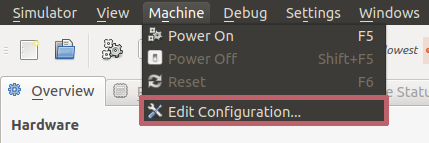
\includegraphics[scale=0.75]{edit_configuration_old}
		\caption{$\mu$MPS2}
		\label{fig:edit_configuration_old}
	\end{subfigure}
	\newline
	\begin{subfigure}[h]{\textwidth}
		\centering
		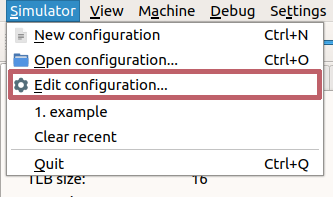
\includegraphics[scale=0.75]{edit_configuration}
		\caption{$\mu$MPS3}
		\label{fig:edit_configuration_new}
	\end{subfigure}
	\caption{Edit Configuration Menu Entry}
	\label{fig:edit_configuration}
\end{figure}

A ``\textit{Clear recent}'' option has been added, an underestimated, yet still useful, function offering the possibility to remove all the used machine configurations from the ``Recent menu'' [\autoref{fig:clear_recent}].
Previously, the only way to do it was by manually editing \texttt{$\sim$/.config/umps3/umps.conf}, not a very practical method to clear the emulator overview.
\begin{figure}[h]
	\centering
	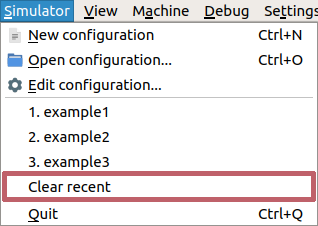
\includegraphics[scale=0.75]{clear_recent}
	\caption{Clear Recent Menu Entry}
	\label{fig:clear_recent}
\end{figure}

\clearpage
The ``\textit{Reset}'' shortcut has been made available in the processor view as well.
This is a convenient option when debugging using only the keyboard, thus allowing the restart of the machine without the need to move between front-end windows [\autoref{fig:reset}].
\begin{figure}[h]
	\centering
	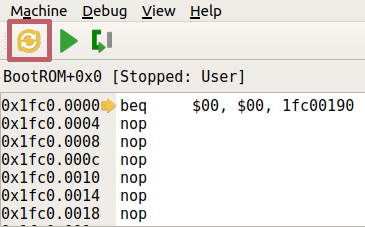
\includegraphics[scale=0.7]{reset}
	\caption{Reset Shortcut}
	\label{fig:reset}
\end{figure}

The \texttt{RAMTOP} value of the machine is now available from the configuration overview [\autoref{fig:ramtop}], increasing the transparency for the user on how the physical memory of $\mu$MPS works [\autoref{chap:physical_memory}].
\begin{figure}[h]
	\centering
	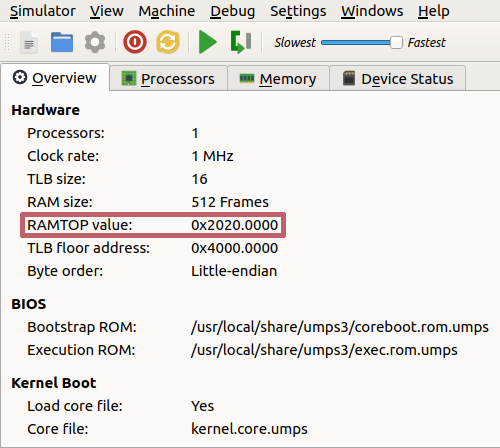
\includegraphics[scale=0.72]{ramtop}
	\caption{\texttt{RAMTOP} value}
	\label{fig:ramtop}
\end{figure}

\chapter{Conclusions}
\lhead[\fancyplain{}{\bfseries\thepage}]{\fancyplain{}{\bfseries\rightmark}}
The $\mu$MPS project was created almost twenty years ago as a didactic support for operating system courses.
Over time, many instructors have chosen it as an aid in their classes, allowing it to reach its initial goal.
However, from the day the last version has been released, educational and technological standards have changed in many ways, and the consideration of it has been dropping to these days.
A refresh of the emulator was needed, in order to renovate the outdated features and reintroduce it to new OS instructors.
Thus, $\mu$MPS3 has been designed and implemented, and describing how this update differs from the previous version is the work of this thesis.

The most changed aspect is, probably, the whole memory system, which has been simplified compared to the original design, aligned to modern management techniques, and, ironically, unintentionally brought back to the original MIPS architecture in various facets.

The internal exception handling system (BIOS routines) has been completely redesigned, facilitating its operation and requiring less work from the students.
By moving some responsibilities from the kernel to the BIOS, the users kernel designing job is simpler and less sophisticated.
This new implementation led also to the modification of the processors initialization process.

From the set of five previously supported devices, the tape is the one which suffered the most the passage of time.
Very few $\mu$MPS users from the current generation of students are aware of how it works or what it even is.
Current hardware like USB sticks or SD cards is surely more appropriate for educational purpose, since a familiar match of what one is working on helps to understand better.
For these reasons, the new class of flash devices has been introduced, filling the need for substituting another outdated view of the project.

Last but not least, the project building process had to be simplified.
It was probably the very first (underestimated) obstacle that students encountered while trying to install $\mu$MPS, and it was based on the GNU Autotools.
The migration to a new, current, building tool like CMake made the whole procedure more linear and pretty straightforward.
The graphical user interface has not been revolutionized, but it has been updated anyway from Qt4 to Qt5 with the addition of a few adjustments.

With this second major revision, the $\mu$MPS project is once again in line with how a proper current operating systems study aid should be structured.

\section{Future Work}
$\mu$MPS is one of those projects where the work to be done is potentially endless.
Uncountable changes are possible, both big or small, in order to enhance the quality of the software.
The most important, obvious or already planned proposal, will be explained in this final part of the thesis, but it is important to remember that no matter how many examples will be given, it will always be a non-exhaustive list.

\subsection{Software Packaging}
Once a software has been released, it has to be distributed to future users.
$\mu$MPS is an open-source project, and its code will be always available in public \textit{Git} \cite{git} repositories like \textit{GitHub} \cite{github}.
This allows it to be always built from source and installed in almost every system.
However, it is always preferable to install software from official repositories when available, since it permits an integrated tracking of installed files and an automatic updates system.
Therefore, the first task after $\mu$MPS3 release is packaging it for Linux distros, to simplify even more its installation process, which will also permit a solid future updates distribution.

\textit{Debian} \cite{debian} is the main distribution for which the software must be packaged, since along with all its derivates it covers the majority of the most popular distros used.
The guidelines of its packaging process are the most stringent, but once the package is complete the porting to other derivates repositories should be straightforward.

The second major distribution that is taking hold in these days is \textit{Arch Linux} \cite{arch_linux}, along with a long list of derivates as well.
The packaging process for this distribution is a lot more simpler than for Debian, and users-produced packages can be uploaded in the dedicated repository at any time in a few steps.
The second version of the software, $\mu$MPS2, has been available in the \textit{AUR} (Arch User Repository) for over a year.

There are obviously a large number of other Linux distributions not based on Debian or Arch, for which the two packaging processes listed before are, then, useless.
Satisfying all the possible Linux ``flavours'' is an almost infinite work, and it is hoped that others will contribute to this cause by creating the package for the distribution they use.

Other possible solutions are distro agnostic packages, like \textit{Flatpak} \cite{flatpak}, \textit{AppImage} \cite{appimage}, and \textit{Snapcraft} \cite{snapcraft}.
They provide a way to distribute software that could run on every system regardless of the distribution used.

\subsection{Persistent Debugging Settings}
Thanks to the advanced debugging support, $\mu$MPS is unique in its kind.
All the related features allow a high-level dismantling of the machine workflow, that enables the user to exactly understand what the emulator is doing or where the code is failing.
Sadly, the settings environment related to a machine that can be created at runtime cannot be saved on the disk, and it is lost when closing the program.

A nice new feature to develop could be linked to this aspect, since storing off all the breakpoints, suspects, targets or all the traced regions set during an hour of debugging could be convenient.
Later in time, one could load the setup previously saved and start debugging from where left off.
Undoubtedly, a cycle of compatibility checks is necessary to avoid loading incompatible debugging settings on a machine.

\subsection{Better Block Devices Creation}
A block device is a type of file which represents a device of some kind internally block-structured.
This means that its data is read or written in it in blocks.
$\mu$MPS supports two types of block devices: disks and flash devices.
During their creation, a certain amount of space is always left blank, not loaded with any information given.
This space is currently filled with empty blocks, all set to the \texttt{0} value.
Consequently, a certain amount of memory is occupied on the real disk, without any useful information to maintain.
By re-designing the creation process, for example by using the \texttt{truncate} function, it would be possible to achieve the same result without filling the actual file on the disk with unnecessary information.
A new implementation has already been proposed, and it should be integrated in a future minor release of $\mu$MPS3.

Furthermore, at the moment, it is possible to write only one file into a newly created flash device.
An update to the creation process of the device should implement also the ability to load multiple files, as it was possible with tapes.

Similarly, disks creation does not allow to load any files into them, but only to generate blank devices.
Along with the suggestions above, the \texttt{umps3-mkdev} utility should be altered to also permit the creation of non-empty disks images.
Due to the physical characteristics of their geometry, this will be a nontrivial task compared to the filling process of flash devices contiguous space.

\begin{thebibliography}{99}
	\addcontentsline{toc}{chapter}{Bibliography}

	\bibitem{chip_1}
	O. Babaoglu, M. Bussan, R. Drummond, F. Schneider,
	\textit{Documentation for the CHIP computer system},
	Department of Computer Science, Cornell University, (Ithaca, NY, USA), Technical Report TR 83-584, December 1983.

	\bibitem{chip_2}
	L. Alvisi, F. Schneider,
	\textit{A graphical interface for CHIP}
	Department of Computer Science, Cornell University, (Ithaca, NY, USA), Technical Report TR 96-1591, June 1996.

	\bibitem{hoca}
	O. Babaoglu, F. Schneider,
	\textit{The HOCA Operating System Specifications},
	Department of Computer Science, Cornell University, (Ithaca, NY, USA), Technical Report TR 83-585, December 1983.

	\bibitem{mps}
	M. Morsiani, R. Davoli,
	\textit{Learning Operating Systems Structure and Implementation through the MPS Computer System Simulator},
	in \textit{The Proceedings of the Thirtieth SIGCSE Technical Symposium on Computer Science Education},
	SIGCSE '99, (New York, NY, USA), pp. 63-67, ACM, March 1999.

	\bibitem{kaya}
	M. Goldweber, R. Davoli, and M. Morsiani,
	\textit{The Kaya OS Project and the $\mu$MPS Hardware Emulator},
	in \textit{Proceedings of the 10th Annual SIGCSE Conference on Innovation and Technology in Computer Science Education},
	ITiCSE '05, (New York, NY, USA), pp. 49–53, ACM, June 2005.

	\bibitem{umps2}
	M. Goldweber, R. Davoli, and T. Jonjic,
	\textit{Supporting Operating Systems Projects Using the $\mu$MPS2 Hardware Simulator},
	in \textit{Proceedings of the 17th ACM Annual Conference on Innovation and Technology in Computer Science Education},
	ITiCSE '12, (New York, NY, USA), pp. 63–68, ACM, July 2012.

	\bibitem{pops}
	M. Goldweber, R. Davoli,
	\textit{$\mu$MPS3 Principles of Operation},
	Lulu Books, 2020.

	\bibitem{old_pops}
	M. Goldweber, R. Davoli,
	\textit{$\mu$MPS2 Principles of Operation},
	Lulu Books, August 2011.

	\bibitem{autotools}
	GNU Project,
	\textit{Autotools},
	\url{https://www.gnu.org/}.

	\bibitem{linux_kernel}
	Linux's Contributors,
	\textit{Linux Kernel},
	\url{https://www.kernel.org/}.

	\bibitem{tjonjic}
	T. Jonjic,
	\textit{Design and Implementation of the $\mu$MPS2 Educational Emulator},
	University of Bologna, 2012.

	\bibitem{papirus}
	Papirus Development Team,
	\textit{Papirus Icon Theme for Linux},
	\url{https://github.com/PapirusDevelopmentTeam/papirus-icon-theme}.

	\bibitem{gpl3}
	Free Software Foundation, Inc.,
	\textit{GNU General Public License Version 3},
	\url{https://www.gnu.org/licenses/gpl-3.0.en.html}.

	\bibitem{inkscape}
	Inkscape's Contributors,
	\textit{The Inkscape Project},
	\url{https://inkscape.org/}.

	\bibitem{ubuntu_mono}
	Canonical Ltd.,
	\textit{Ubuntu font},
	\url{https://design.ubuntu.com/font/}.

	\bibitem{git}
	Git's Contributors,
	\textit{Git},
	\url{https://git-scm.com/}.

	\bibitem{github}
	Microsoft Corporation,
	\textit{GitHub},
	\url{https://github.com/}.

	\bibitem{debian}
	Debian Project,
	\textit{Debian},
	\url{https://www.debian.org/}.

	\bibitem{arch_linux}
	Arch Linux's Contributors,
	\textit{Arch Linux},
	\url{https://www.archlinux.org/}.

	\bibitem{flatpak}
	Flatpak's Contributors,
	\textit{Flatpak},
	\url{https://www.flatpak.org/}.

	\bibitem{appimage}
	Simon Peter,
	\textit{AppImage},
	\url{https://appimage.org/}.

	\bibitem{snapcraft}
	Canonical Ltd.,
	\textit{Snapcraft},
	\url{https://snapcraft.io/}.

\end{thebibliography}

\chapter*{Acknowledgements}
Thanks to my mentors, Prof. Renzo Davoli and Prof. Michael Goldweber, who patiently guided me through the development of the project and the drafting of this document with invaluable advice.
Their contagious passion in Operating Systems and everything related to it made the final part of my course of study the most enjoyable one.

Special thanks to Jasmine, who is, de facto, the third supervisor of the thesis.

\end{document}
